\documentclass{article}[12pt]
\usepackage{amsmath}
\usepackage{array}
\usepackage{amsfonts}
\usepackage{graphicx}
\usepackage{booktabs}
\usepackage{tikz}
\usetikzlibrary{arrows.meta, positioning, calc, shapes.geometric}
\usepackage[table]{xcolor}
\usepackage{array, rotating, colortbl, xcolor, booktabs}
\usepackage{adjustbox}
\usepackage[left=3cm, right=2cm, top=2cm, bottom=2cm]{geometry}


\newcommand{\cmdA}{\ensuremath{\mathsf{A}}} % Command: Attack
\newcommand{\cmdR}{\ensuremath{\mathsf{R}}} % Command: Retreat
\newcommand{\loyal}{\ensuremath{\mathcal{L}}}
\newcommand{\traitor}{\ensuremath{\mathcal{T}}}
\newcommand{\gen}[1]{\ensuremath{G_{#1}}}

% TikZ styles
\tikzstyle{general} = [circle, draw, minimum size=0.9cm, font=\small]
\tikzstyle{messageA} = [-{Stealth[length=2.5mm, width=2mm]}, blue, thick] % Blue for Attack
\tikzstyle{messageR} = [-{Stealth[length=2.5mm, width=2mm]}, red, thick]  % Red for Retreat
\tikzstyle{nodeLabel} = [font=\scriptsize, right=1pt]

% --- Definitions for storing and measuring the table and labels ---
\newsavebox{\mainTableBox}
\newlength{\mainTableHeight}
\newlength{\mainTableWidth}
\newlength{\senderLabelAreaHeight}
\newlength{\majorityLabelAreaHeight}


\begin{document}

\section*{Byzantine Generals: OM(2) with Traitor Commander}
$N=7$ generals, $t=2$ traitors. Commander $\gen{0}$ is a traitor.
\begin{itemize}
    \item Commander: $\gen{0}(\traitor)$
    \item Lieutenants: $\gen{1}(\traitor)$, $\gen{2}(\loyal)$, $\gen{3}(\loyal)$, $\gen{4}(\loyal)$, $\gen{5}(\loyal)$, $\gen{6}(\loyal)$
\end{itemize}
Traitor Strategies:
\begin{itemize}
    \item $\gen{0}(\traitor)$: Sends \cmdA{} to $\gen{2},\gen{4},\gen{6}$. Sends \cmdR{} to $\gen{1},\gen{3},\gen{5}$.
    \item $\gen{1}(\traitor)$: (Received \cmdR{} from $\gen{0}$) When sending/relaying: sends \cmdA{} to $\gen{2},\gen{4},\gen{6}$; sends \cmdR{} to $\gen{3},\gen{5}$.
\end{itemize}

\subsection*{Round 1: Commander $\gen{0}$ (Traitor) Sends Commands}
$\gen{0}$ sends its chosen messages to the lieutenants.
\begin{figure}[htb]
\centering
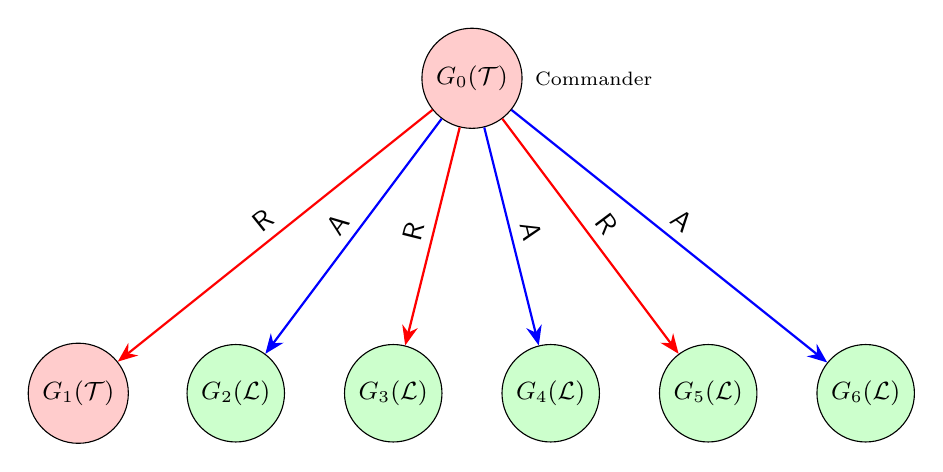
\begin{tikzpicture}[scale=1, transform shape]
    % Commander
    \node[general, fill=red!20, label={[nodeLabel]right:{Commander}}] (g0) at (0,4) {$\gen{0}(\traitor)$};

    % Lieutenants
    \node[general, fill=red!20] (g1) at (-5,0) {$\gen{1}(\traitor)$};
    \node[general, fill=green!20] (g2) at (-3,0) {$\gen{2}(\loyal)$};
    \node[general, fill=green!20] (g3) at (-1,0) {$\gen{3}(\loyal)$};
    \node[general, fill=green!20] (g4) at (1,0) {$\gen{4}(\loyal)$};
    \node[general, fill=green!20] (g5) at (3,0) {$\gen{5}(\loyal)$};
    \node[general, fill=green!20] (g6) at (5,0) {$\gen{6}(\loyal)$};

    % Messages from G0
    \draw[messageR] (g0) -- (g1) node[midway, above, sloped, black]{\cmdR}; % G0 to G1 (Traitor)
    \draw[messageA] (g0) -- (g2) node[midway, above, sloped, black]{\cmdA}; % G0 to G2 (Loyal)
    \draw[messageR] (g0) -- (g3) node[midway, above, sloped, black]{\cmdR}; % G0 to G3 (Loyal)
    \draw[messageA] (g0) -- (g4) node[midway, above, sloped, black]{\cmdA}; % G0 to G4 (Loyal)
    \draw[messageR] (g0) -- (g5) node[midway, above, sloped, black]{\cmdR}; % G0 to G5 (Loyal)
    \draw[messageA] (g0) -- (g6) node[midway, above, sloped, black]{\cmdA}; % G0 to G6 (Loyal)
\end{tikzpicture}
\caption{Round 1: Traitor Commander $\gen{0}$ sends messages.}

\begin{center}
\vspace{1em} % Add some vertical space
\renewcommand{\arraystretch}{1.5}
\setlength{\tabcolsep}{6pt} % Adjusted
\begin{tabular}{c|c|c|c|c|c}
    \hline
    \textbf{$\gen{1}(\traitor)$} & \textbf{$\gen{2}(\loyal)$} & \textbf{$\gen{3}(\loyal)$} & \textbf{$\gen{4}(\loyal)$} & \textbf{$\gen{5}(\loyal)$} & \textbf{$\gen{6}(\loyal)$} \\
    \hline
    \cellcolor{yellow!30}\textbf{\textcolor{red}{\cmdR}} & & & & & \\
    \hline
     & \cellcolor{yellow!30}\textbf{\textcolor{blue}{\cmdA}} & & & & \\
    \hline
     & & \cellcolor{yellow!30}\textbf{\textcolor{red}{\cmdR}} & & & \\
    \hline
     & & & \cellcolor{yellow!30}\textbf{\textcolor{blue}{\cmdA}} & & \\
    \hline
     & & & & \cellcolor{yellow!30}\textbf{\textcolor{red}{\cmdR}} & \\
    \hline
     & & & & & \cellcolor{yellow!30}\textbf{\textcolor{blue}{\cmdA}} \\
    \hline
\end{tabular}
\par\vspace{0.3em}
{\scriptsize
The grid above shows the initial values $v_i$ that each lieutenant $\gen{i}$ (represented by row and column headers) receives from Commander $\gen{0}$ and stores. This value is placed on the diagonal cell $(\gen{i}, \gen{i})$. Off-diagonal cells are empty, to be filled by messages exchanged between lieutenants in later algorithm phases (e.g., OM(m-1) rounds).
}
\end{center}

\end{figure}

\begin{figure}[htb]
\centering
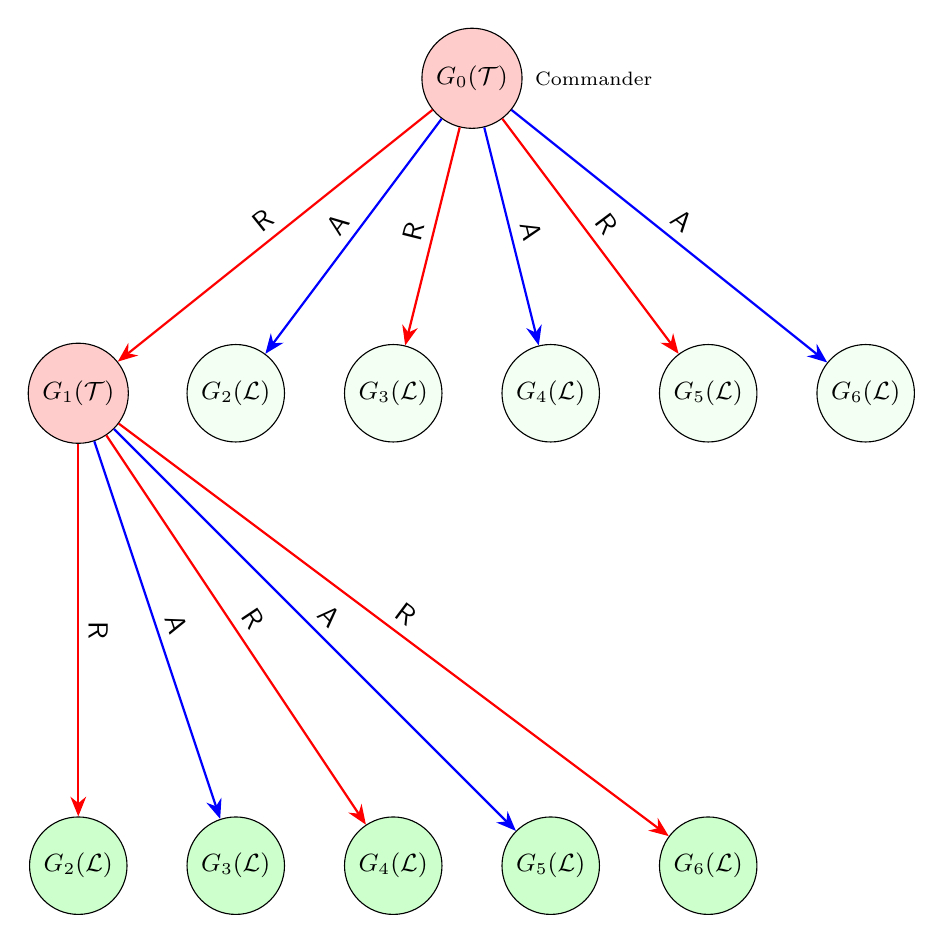
\begin{tikzpicture}[scale=1, transform shape]
    % Commander
    \node[general, fill=red!20, label={[nodeLabel]right:{Commander}}] (g0) at (0,4) {$\gen{0}(\traitor)$};

    % Lieutenants (Level 1)
    \node[general, fill=red!20] (g1) at (-5,0) {$\gen{1}(\traitor)$};
    \node[general, fill=green!5] (g2) at (-3,0) {$\gen{2}(\loyal)$};
    \node[general, fill=green!5] (g3) at (-1,0) {$\gen{3}(\loyal)$};
    \node[general, fill=green!5] (g4) at (1,0) {$\gen{4}(\loyal)$};
    \node[general, fill=green!5] (g5) at (3,0) {$\gen{5}(\loyal)$};
    \node[general, fill=green!5] (g6) at (5,0) {$\gen{6}(\loyal)$};

    % Messages from Commander (Level 1 edges)
    \draw[messageR] (g0) -- (g1) node[midway, above, sloped, black]{\cmdR};
    \draw[messageA] (g0) -- (g2) node[midway, above, sloped, black]{\cmdA};
    \draw[messageR] (g0) -- (g3) node[midway, above, sloped, black]{\cmdR};
    \draw[messageA] (g0) -- (g4) node[midway, above, sloped, black]{\cmdA};
    \draw[messageR] (g0) -- (g5) node[midway, above, sloped, black]{\cmdR};
    \draw[messageA] (g0) -- (g6) node[midway, above, sloped, black]{\cmdA};

    % Second Level: Lieutenants communicating with each other (add this section)
    \begin{scope}[yshift=-3cm] % Shift downward for the second layer
        % New nodes (spaced horizontally like the first layer)
        \node[general, fill=green!20] (g2a) at (-5,-3) {$\gen{2}(\loyal)$}; % Match g1's x-position
        \node[general, fill=green!20] (g3a) at (-3,-3) {$\gen{3}(\loyal)$}; % Match g2's x-position
        \node[general, fill=green!20] (g4a) at (-1,-3) {$\gen{4}(\loyal)$};
        \node[general, fill=green!20] (g5a) at (1,-3) {$\gen{5}(\loyal)$};
        \node[general, fill=green!20] (g6a) at (3,-3) {$\gen{6}(\loyal)$};
    
        % Draw edges between lieutenants (example: traitor g1 sends conflicting messages)
        \draw[messageR] (g1) -- (g2a) node[midway, above, sloped, black]{\cmdR};

        \draw[messageA] (g1) -- (g3a) node[midway, above, sloped, black]{\cmdA};
        \draw[messageR] (g1) -- (g4a) node[midway, above, sloped, black]{\cmdR};
        \draw[messageA] (g1) -- (g5a) node[midway, above, sloped, black]{\cmdA};
        \draw[messageR] (g1) -- (g6a) node[midway, above, sloped, black]{\cmdR};
    \end{scope}
\end{tikzpicture}
\caption{Round 2: Traitor Lieutenant $\gen{0}$ sends conflicting messages. Lieutenants now communicate with each other.}

% --- Step 1: Typeset the main data table into a savebox to measure its dimensions ---
\sbox{\mainTableBox}{%
  \renewcommand{\arraystretch}{1.3}%
  \setlength{\tabcolsep}{12pt}%
  \begin{tabular}{c|c|c|c|c|c}
    \textbf{} & \textbf{$\gen{2}$} & \textbf{$\gen{3}$} & \textbf{$\gen{4}$} & \textbf{$\gen{5}$} & \textbf{$\gen{6}$} \\
    \hline

    \textbf{$\gen{2}$} & \cellcolor{yellow!30}\textbf{\textcolor{red}{R}} & \cellcolor{red!20}\textcolor{red}{R} & \cellcolor{red!20}\textcolor{red}{R} & \cellcolor{red!20}\textcolor{red}{R} & \cellcolor{red!20}\textcolor{red}{R} \\
    \textbf{$\gen{3}$} & \cellcolor{blue!20}\textcolor{blue}{A} & \cellcolor{yellow!30}\textbf{\textcolor{blue}{A}} & \cellcolor{blue!20}\textcolor{blue}{A} & \cellcolor{blue!20}\textcolor{blue}{A} & \cellcolor{blue!20}\textcolor{blue}{A} \\
    \textbf{$\gen{4}$} & \cellcolor{red!20}\textcolor{red}{R} & \cellcolor{red!20}\textcolor{red}{R} & \cellcolor{yellow!30}\textbf{\textcolor{red}{R}} & \cellcolor{red!20}\textcolor{red}{R} & \cellcolor{red!20}\textcolor{red}{R} \\
    \textbf{$\gen{5}$} & \cellcolor{blue!20}\textcolor{blue}{A} & \cellcolor{blue!20}\textcolor{blue}{A} & \cellcolor{blue!20}\textcolor{blue}{A} & \cellcolor{yellow!30}\textbf{\textcolor{blue}{A}} & \cellcolor{blue!20}\textcolor{blue}{A} \\
    \textbf{$\gen{6}$} & \cellcolor{red!20}\textcolor{red}{R} & \cellcolor{red!20}\textcolor{red}{R} & \cellcolor{red!20}\textcolor{red}{R} & \cellcolor{red!20}\textcolor{red}{R} & \cellcolor{yellow!30}\textbf{\textcolor{red}{R}} \\
    \hline\hline
    \textbf{Majority} & \cellcolor{red!75}\textbf{\textcolor{white}{R}}  & \cellcolor{red!75}\textbf{\textcolor{white}{R}}  & \cellcolor{red!75}\textbf{\textcolor{white}{R}}  & \cellcolor{red!75}\textbf{\textcolor{white}{R}} & \cellcolor{red!75}\textbf{\textcolor{white}{R}} \\
  \end{tabular}%
}
% --- Step 2: Get the measured height and width of the saved table ---
\setlength{\mainTableHeight}{\dimexpr\ht\mainTableBox+\dp\mainTableBox\relax}
\setlength{\mainTableWidth}{\wd\mainTableBox}


% --- Step 3: Calculate proportional heights for Sender and Majority label areas ---
% Sender area corresponds to 6 out of 7 conceptual rows.
% Majority area corresponds to 1 out of 7 conceptual rows.
\setlength{\senderLabelAreaHeight}{\dimexpr 6\mainTableHeight / 7 \relax}
\setlength{\majorityLabelAreaHeight}{\dimexpr \mainTableHeight - \senderLabelAreaHeight \relax} % Ensures sum is exactly \mainTableHeight

\centering
{\large \textbf{Receiver}\par}
\vspace{0.5em}


% --- Step 4: Assemble the labels and table using adjustbox for vertical centering ---
\newlength{\labelcolwidth} % Define a new length
\settowidth{\labelcolwidth}{\textbf{Majority}} % Set it to the width of "Majority"

\begin{tabular}{@{}c@{\hspace{1em}}c@{}}
  \adjustbox{valign=c}{% Vertically center the entire label column box
    \parbox[t][\mainTableHeight][c]{\labelcolwidth}{ % Use \labelcolwidth for the outer parbox width
      \centering % Horizontally center the inner parboxes (Sender & Majority areas)
      \parbox[c][\senderLabelAreaHeight][c]{\labelcolwidth}{ % Sender area, use \labelcolwidth
        \centering\rotatebox[origin=c]{90}{\large\textbf{Sender}}
      }
    }
  }
  &
  \adjustbox{valign=c}{\usebox{\mainTableBox}} % Use the saved (and measured) table, vertically centered
\end{tabular}


    \vspace{0.7em}

    {\small
    \textbf{Legend:} Rows (left) are senders, columns (top) are receivers. Each cell shows the message the sender tells the receiver that it received from $\gen{1}$. Yellow diagonal: sender's own message from $\gen{1}$. Blue = Attack (A), Red = Retreat (R).
    }

    \begin{center}
    \vspace{1em} % Add some vertical space
    \renewcommand{\arraystretch}{1.5}
    \setlength{\tabcolsep}{6pt} % Adjusted
    \begin{tabular}{c|c|c|c|c|c}
        \hline
        \textbf{$\gen{1}(\traitor)$} & \textbf{$\gen{2}(\loyal)$} & \textbf{$\gen{3}(\loyal)$} & \textbf{$\gen{4}(\loyal)$} & \textbf{$\gen{5}(\loyal)$} & \textbf{$\gen{6}(\loyal)$} \\
        \hline
        \cellcolor{yellow!30}\textbf{\textcolor{red}{\cmdR}} & \cellcolor{red!75}\textbf{\textcolor{white}{R}} & \cellcolor{red!75}\textbf{\textcolor{white}{R}} & \cellcolor{red!75}\textbf{\textcolor{white}{R}} & \cellcolor{red!75}\textbf{\textcolor{white}{R}} & \cellcolor{red!75}\textbf{\textcolor{white}{R}} \\
        \hline
        & \cellcolor{yellow!30}\textbf{\textcolor{blue}{\cmdA}} & & & & \\
        \hline
        & & \cellcolor{yellow!30}\textbf{\textcolor{red}{\cmdR}} & & & \\
        \hline
        & & & \cellcolor{yellow!30}\textbf{\textcolor{blue}{\cmdA}} & & \\
        \hline
        & & & & \cellcolor{yellow!30}\textbf{\textcolor{red}{\cmdR}} & \\
        \hline
        & & & & & \cellcolor{yellow!30}\textbf{\textcolor{blue}{\cmdA}} \\
        \hline
    \end{tabular}
    \par\vspace{0.3em}
    {\scriptsize
    The grid above shows the initial values $v_i$ that each lieutenant $\gen{i}$ (represented by row and column headers) receives from Commander $\gen{0}$ and stores. This value is placed on the diagonal cell $(\gen{i}, \gen{i})$. Off-diagonal cells are empty, to be filled by messages exchanged between lieutenants in later algorithm phases (e.g., OM(m-1) rounds).
    }
\end{center}


\end{figure}


\end{document}